\documentclass{article}

\usepackage[a4paper, total={6.5in, 11in}]{geometry}
\usepackage{graphicx}
\usepackage{subfig}
\usepackage{gensymb}
\usepackage{hyperref}
\graphicspath{{titech/CSC.T463.ComputerGraphics/h7/}}

\usepackage{latex/common}

\title{Computer Graphics 2021 - Assignment 7}
\author{Sixue Wang\\21M30927\\Tokyo Institute of Technology}

\begin{document}

\maketitle


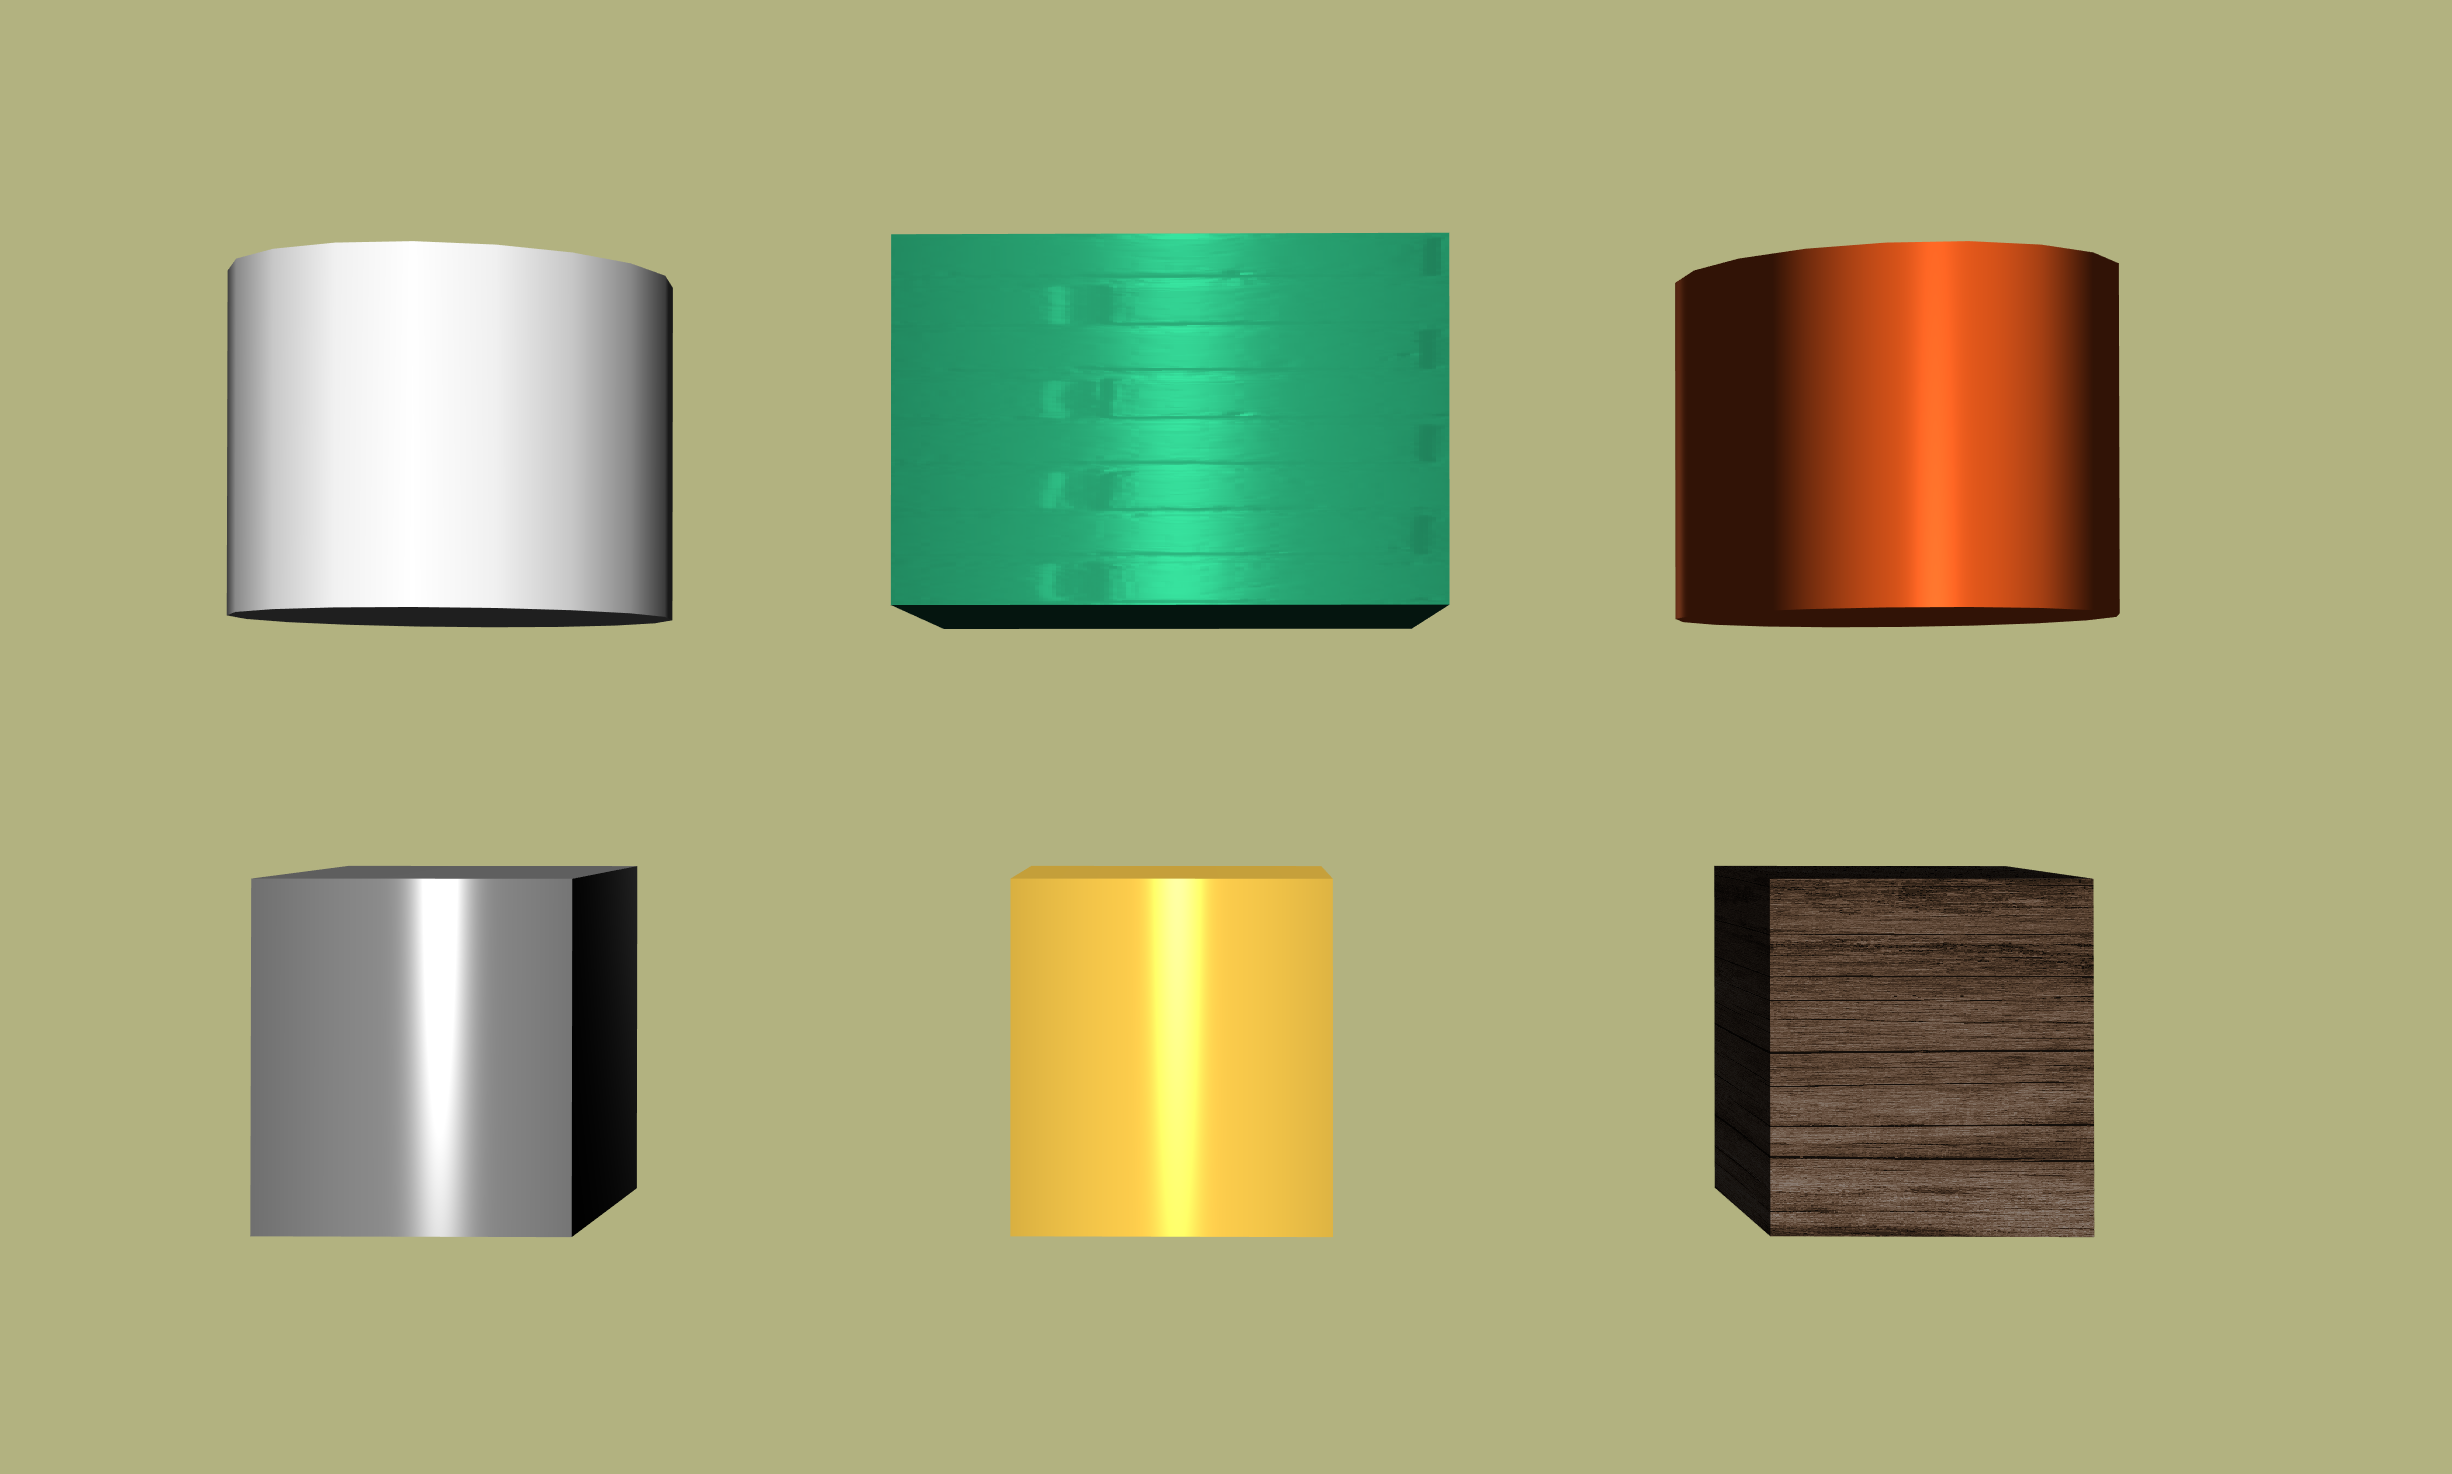
\includegraphics[width=1\textwidth]{h7.png}

\section{}

The light color is white under D65 light environment.

\subsection*{chalk}

For white chalk, we don't need any texture but set color to white directly.
One of most significantly characteristic of chalk is that the specular reflection is almost none.
So we reuse ``spot'' shard but remove specular reflection part. We also change the weight contribution of ambient reflection to 0.1 and diffuse reflection to 0.9.

\begin{equation*}
  (ambient + diffuse) * lightColor * objColor
\end{equation*}
\begin{equation*}
  (0.1 + 0.9*max(normalDir \cdot lightDir, 0)) * white * white
\end{equation*}

\subsection*{brick}

Let's consider color and the contribution of each reflection component first. We set brick color to (0.199, 0.819, 0.572) according to the \#74 pigment. Unlike chalk, we enable specular reflection for brick. But the major of reflection of brick is still diffuse reflection.

\begin{equation*}
  (ambient + 0.7*diffuse + 0.3*specular) * lightColor * objColor
\end{equation*}
\begin{equation*}
  (0.1 + 0.9*max(normalDir \cdot lightDir, 0) + 0.3*max(reflectDir \cdot viewDir)) * white * (0.199, 0.819, 0.572)
\end{equation*}
Now let's consider the brick texture together. One simplest way is mixing the original color with ``Brick.png'' texture
\begin{equation*}
  (ambient + 0.7*diffuse + 0.3*specular) * lightColor * mix(objColor, textureColor, 0.2)
\end{equation*}
We also found that bump mapping provide better shadows on contours by modifing normalDir.
\begin{equation*}
  normalDir = normalize(normal + 0.15 * textureColor*2-1)
\end{equation*}

\subsection*{copper}
Fortunately, we can find copper parameters on this \href{http://www.it.hiof.no/~borres/j3d/explain/light/p-materials.html}{website}.
$$
  \begin{bmatrix}
    ambient color  & = & 0.19125 & 0.0735 & 0.0225 \\
    diffuse color  & = & 0.7038 & 0.27048 & 0.0828 \\
    specular color & = & 0.256777 & 0.137622 & 0.086014 \\
    shine          & = & 12.8
  \end{bmatrix}
$$
which means we neither need to set color nor texture. The final reflection is calculated by the following equation:
$$
  (ambient + diffuse + specular) * lightColor
$$
where
\begin{itemize}
  \item $ambient = (0.19125, 0.0735, 0.0225)$
  \item $diffuse = max(normalDir \cdot lightDir, 0) * (0.7038, 0.27048, 0.0828)$
  \item $specular = pow(max(reflectDir \cdot viewDir, 0.0), 12.8) * (0.256777, 0.137622, 0.086014)$
\end{itemize}

\section{}

\subsection*{plastic and gold}
We can also define a white plastic and gold object by a similar way with copper:

Plastic:
$$
  \begin{bmatrix}
    ambient color  & = & 0. & 0.& 0.\\
    diffuse color  & = & 0.55 & 0.55 & 0.55 \\
    specular color & = & 0.7 & 0.7 & 0.7 \\
    shine          & = & 32
  \end{bmatrix}
$$

Gold:
$$
  \begin{bmatrix}
    ambient color  & = & 0.25 & 0.2 & 0.07 \\
    diffuse color  & = & 0.75 & 0.61 & 0.23 \\
    specular color & = & 0.63 & 0.65 & 0.37 \\
    shine          & = & 51.2
  \end{bmatrix}
$$

\subsection*{wood}
Firstly, We downloaded a wood texture then we tried to fine-tune factors of the reflection model. Personally, we think there is no specular reflection and we also decrease diffuse reflection.
\begin{equation*}
  (ambient + diffuse) * lightColor * textureColor
\end{equation*}
\begin{equation*}
  (0.1 + 0.5*max(normalDir \cdot lightDir, 0)) * white * textureColor
\end{equation*}


\end{document}
